\section{Combined Loading}

\subsection{Types of Loading Summary}

If a loading results in more than one type of stress, the total stress in a cross-section can be calculated by adding the individual stresses together (superposition). A review of the stresses covered in this course is below:

\begin{figure*}[!h]
\centering
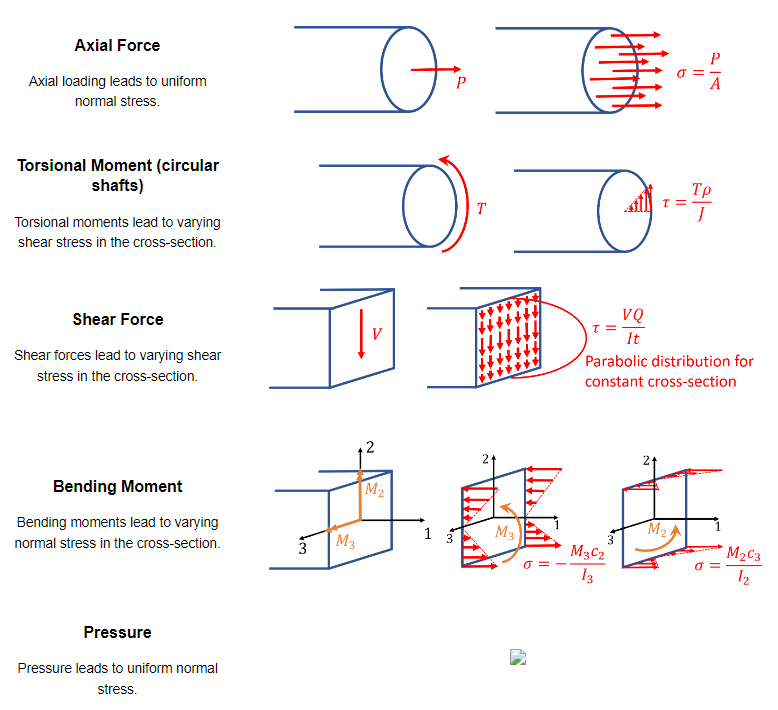
\includegraphics[angle=0, width=6in]{Combined Loading-Figures/LoadTypes.png}
\vspace{-2mm}
\caption{\small From reference pages}
\vspace{-3mm}
\label{Fig:LoadTypes}
\end{figure*}

\subsection{\blue{Stress Under Combined Loads}}

The goal in combined loading is to determine the stresses at a point in a slender structural member subjected to arbitrary loadings. A cross-section is cut through the point of interest and the internal loading/moments are evaluated at the centroid of the section to maintain equilibrium. This internal system of loading will consist of three force components and three couple vectors (moments). To determine the stress distribution at the point, the principle of superposition is applied.

\begin{figure*}[!h]
\centering
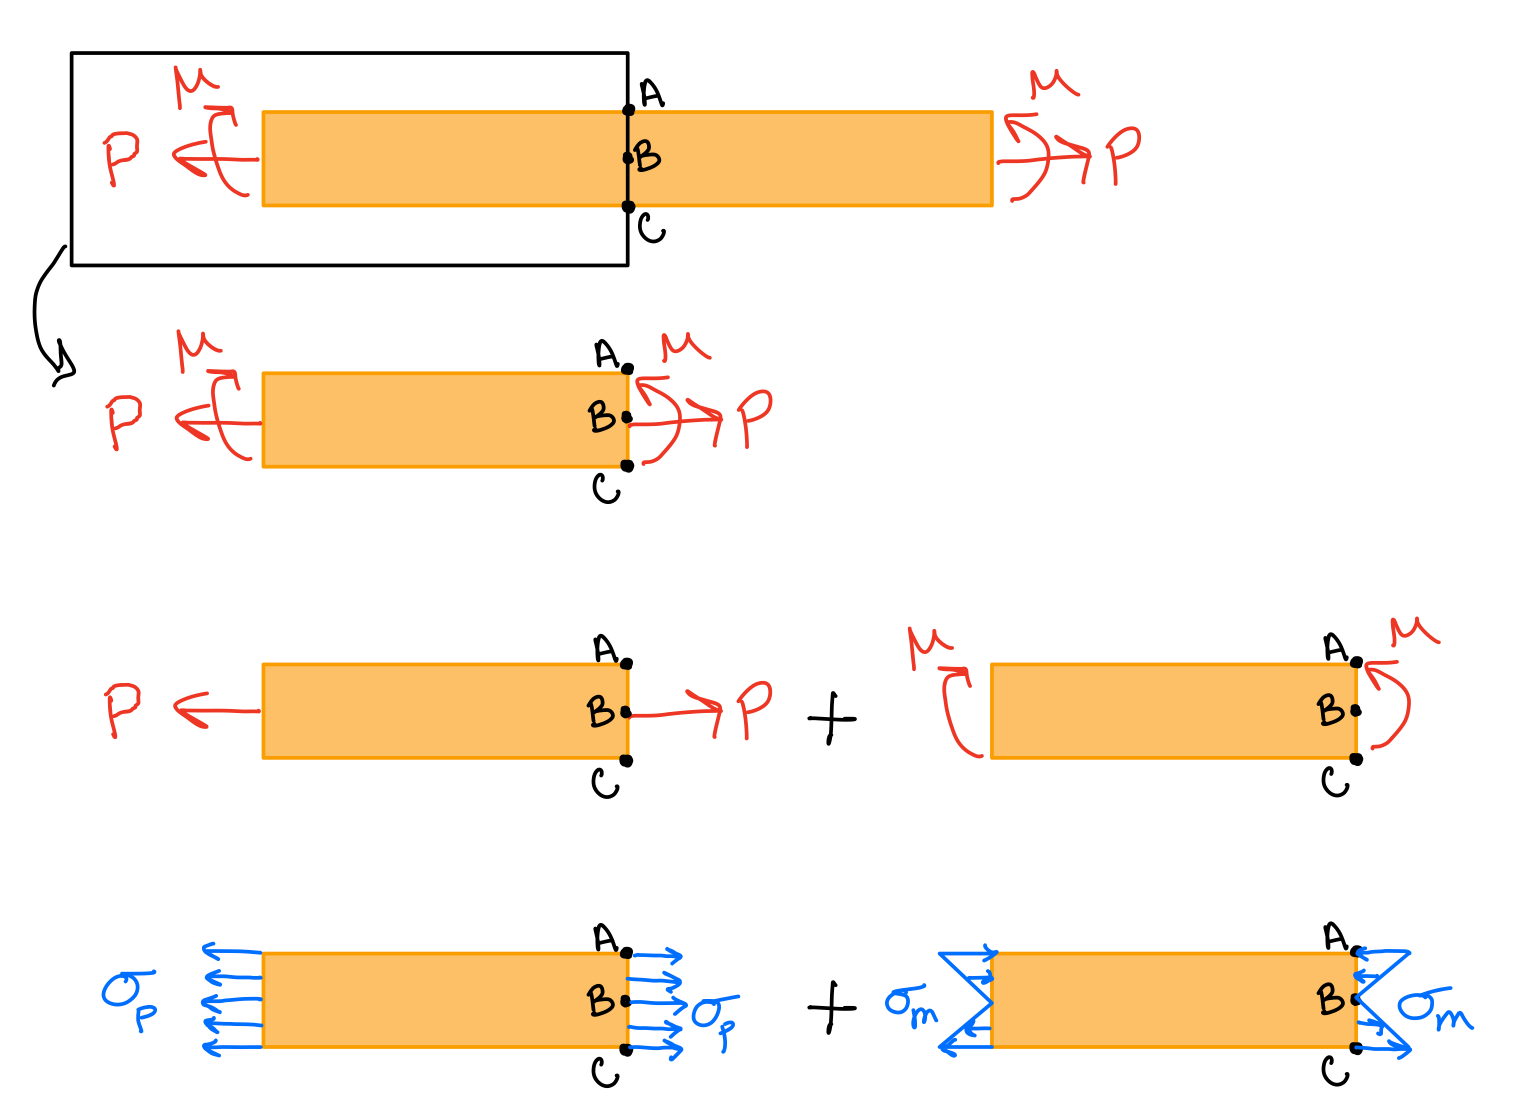
\includegraphics[angle=0, width=4in]{Combined Loading-Figures/Superposition.png}
\vspace{-2mm}
\caption{\small \blue{Taken from TAM251 Lecture Notes - L8S17-18}}
\vspace{-3mm}
\label{Fig:Superposition}
\end{figure*}

\noindent \textbf{Combined Loading Summary:}
\begin{itemize}
    \item Axial force and in-plane couple vectors (moments) contribute to the normal stress distribution in the section.
    \item Shear forces and the twisting couple vector (moment) contribute to the shear stress distribution in the section.
\end{itemize}

\cyan{BSM: a summary of steps to solve these problems might be nice to include here. I teach students to tackle these problems by dividing them into 3 steps: 1) find internal forces/moments in a section of interest, 2) calculate all the stresses acting at a specific point within that section, 3) add up like stresses (matching subscripts) to find the total stress state (superposition)}